%% ============================================================
%%  Care+ Academic Poster  –  A0 Landscape
%%  Sunway College Kathmandu / BCU — Innovation Project 2026
%% ============================================================
\documentclass[final]{beamer}

\usepackage[size=a0, orientation=landscape, scale=1.18]{beamerposter}

%% ── Font ─────────────────────────────────────────────────────
\usepackage[scaled]{helvet}
\renewcommand{\familydefault}{\sfdefault}
\usepackage[T1]{fontenc}
\usepackage[utf8]{inputenc}
\usepackage{microtype}

%% ── Packages ─────────────────────────────────────────────────
\usepackage{graphicx}
\usepackage{colortbl}
\usepackage{array}
\usepackage{tabularx}
\usepackage{xcolor}
\usepackage{tikz}
\usepackage[most]{tcolorbox}
\usepackage{enumitem}
\usepackage{ragged2e}

%% ── Beamer background ────────────────────────────────────────
\usetheme{default}
\setbeamertemplate{navigation symbols}{}
\definecolor{posterbg}{HTML}{F0F2F7}
\setbeamercolor{background canvas}{bg=posterbg}

%% ── Colour palette ───────────────────────────────────────────
\definecolor{navyblue}{HTML}{1A3A6E}
\definecolor{midblue}{HTML}{2563A8}
\definecolor{teal}{HTML}{1E6B8A}
\definecolor{lightblue}{HTML}{E8EEFF}
\definecolor{accentyellow}{HTML}{F4C842}
\definecolor{sdg3col}{HTML}{4C9B4F}
\definecolor{sdg9col}{HTML}{E07820}
\definecolor{sdg10col}{HTML}{D01070}
\definecolor{rowA}{HTML}{FFFFFF}
\definecolor{rowB}{HTML}{EEF1FB}
\definecolor{tableheadbg}{HTML}{1A3A6E}
\definecolor{bordergrey}{HTML}{C0C8D8}

%% ── Section box style ────────────────────────────────────────
\tcbset{
  posterbox/.style={
    enhanced,
    colback=white,
    colframe=navyblue,
    coltitle=white,
    colbacktitle=navyblue,
    fonttitle=\bfseries\large,
    arc=4mm,
    boxrule=1pt,
    toptitle=1.8mm, bottomtitle=1.8mm,
    top=2mm, bottom=2mm, left=4mm, right=4mm,
    drop shadow={black!45!white},
  }
}

%% ── List style ───────────────────────────────────────────────
\setlist[itemize]{
  leftmargin=1.4em, itemsep=3pt, topsep=2pt, parsep=0pt,
  label=\textcolor{navyblue}{\textbullet}
}

%% ── Flow step ────────────────────────────────────────────────
\newcommand{\flowstep}[2]{%
  \vspace{2pt}\noindent
  \begin{tikzpicture}[baseline=(n.base)]
    \node[circle, fill=navyblue, text=white,
          inner sep=0pt, minimum size=22pt,
          font=\bfseries\normalsize] (n) {#1};
  \end{tikzpicture}%
  \hspace{6pt}{\normalsize #2}\par
}

%% ── Result bar ───────────────────────────────────────────────
\newcommand{\resultbar}[3]{%
  \vspace{2pt}
  {\normalsize\textbf{#1}}\par\vspace{3pt}
  \begin{tikzpicture}
    \fill[bordergrey]  (0,0) rectangle (30cm, 0.6cm);
    \fill[#3]          (0,0) rectangle (#2*0.30cm, 0.6cm);
    \node[anchor=east, text=white, font=\small\bfseries]
      at (#2*0.30cm - 0.15cm, 0.3cm) {#2\%};
  \end{tikzpicture}\par\vspace{4pt}
}

%% ── Persona card ─────────────────────────────────────────────
\newcommand{\persona}[3]{%
  \begin{tcolorbox}[
    enhanced, colback=lightblue, colframe=navyblue,
    leftrule=5pt, toprule=0.5pt, bottomrule=0.5pt, rightrule=0.5pt,
    arc=2mm, top=2mm, bottom=2mm, left=4mm, right=4mm,
  ]
    {\bfseries\normalsize\textcolor{navyblue}{#1}}\par\vspace{1pt}
    {\small #2 \textit{--- #3}}
  \end{tcolorbox}\vspace{3pt}
}

%% ── Milestone node ───────────────────────────────────────────
\newcommand{\msnode}[3]{%
  \begin{tcolorbox}[colback=lightblue, colframe=navyblue,
    arc=3mm, boxrule=1pt, top=3mm, bottom=3mm, halign=center]
    {\fontsize{26}{28}\selectfont\bfseries\textcolor{navyblue}{#1}}\par\vspace{2pt}
    {\small\bfseries #2}\par\vspace{1pt}
    {\footnotesize\textit{#3}}
  \end{tcolorbox}
}

%% ============================================================
\begin{document}
\begin{frame}[t]{}

%% ── HEADER ───────────────────────────────────────────────────
\begin{tcolorbox}[
  enhanced, colback=posterbg, colframe=posterbg,
  arc=0mm, boxrule=0pt,
  top=1mm, bottom=1mm, left=0mm, right=0mm,
]
  \begin{columns}[c]

    %% LEFT: Sunway + BCU combined logo
    \begin{column}{0.18\linewidth}
      \centering
      
\includegraphics[height=5.2cm, keepaspectratio]{sunway_bcu_combined.png}
    \end{column}

    %% CENTRE: Title + Authors
    \begin{column}{0.64\linewidth}
      \centering
      {\color{navyblue}\fontsize{46}{52}\selectfont\bfseries
        CarePlus: A Privacy-First AI \& IoT Healthcare Companion\\[2pt]
        for Elderly Home Care in Nepal}\\[7pt]
      {\color{midblue}\fontsize{24}{28}\selectfont\bfseries
        Prashant Adhikari \mdseries\textcolor{teal}{(26140508)}\bfseries\,\textbullet\,
        Adit Bhattarai \mdseries\textcolor{teal}{(26140437)}\bfseries\,\textbullet\,
        Hritik Shrestha \mdseries\textcolor{teal}{(26140472)}\bfseries\,\textbullet\,
        Rakesh KC \mdseries\textcolor{teal}{(26140513)}}\\[4pt]
      {\fontsize{18}{22}\selectfont\itshape
        Team Git Force --- Sunway College Kathmandu, Nepal, in academic
        partnership with Birmingham City University}
    \end{column}

    %% RIGHT: RAIN logo
    \begin{column}{0.18\linewidth}
      \centering
      
\includegraphics[height=5.2cm, keepaspectratio]{rain_logo.png}
    \end{column}

  \end{columns}
\end{tcolorbox}

%% thin navy rule under header
\textcolor{navyblue}{\rule{\linewidth}{2.2pt}}
\vspace{0.5mm}

%% ── THREE COLUMNS ────────────────────────────────────────────
\begin{columns}[t, totalwidth=\linewidth]

%% ════════════════════════════════════════
%%  COLUMN 1
%% ════════════════════════════════════════
\begin{column}{0.315\linewidth}
\vspace{3mm}

%% Motivation
\begin{tcolorbox}[posterbox, title={MOTIVATION}]
  Nepal's ageing population faces a critical care gap as youth emigrate
  abroad. Existing digital health tools are \textbf{English-only,
  cloud-dependent,} and focused on hospital booking, not ongoing home care.
  \begin{itemize}
    \item Elderly patients miss medicines; emotional states go unmonitored.
    \item Remote guardians rely entirely on daily phone calls.
    \item Inconsistent internet makes cloud services unreliable in rural Nepal.
    \item No affordable, Nepali-language AI companion exists for this demographic.
  \end{itemize}
\end{tcolorbox}

\vspace{3mm}

%% Introduction
\begin{tcolorbox}[posterbox, title={INTRODUCTION}]
  \begin{itemize}
    \item \textbf{Goal:} A privacy-first, local-AI healthcare companion for
      elderly Nepali speakers at home.
    \item \textbf{Built:} Raspberry Pi edge device running Whisper STT,
      Gemma LLM, and Piper TTS, paired with a Bun + Express cloud backend,
      mobile app, and web dashboard.
    \item \textbf{Team:} Team Git Force --- four students at Sunway College
      Kathmandu with expertise in AI, IoT, and human-centred design.
    \item \textbf{Approach:} Design Thinking + Agile across four sprints.
  \end{itemize}
\end{tcolorbox}

\vspace{3mm}

%% Use Case Diagram (replaces narrative personas with a concrete diagram)
\begin{tcolorbox}[posterbox, title={WHO USES CARE+ --- USE CASE DIAGRAM}]
  \begin{center}
    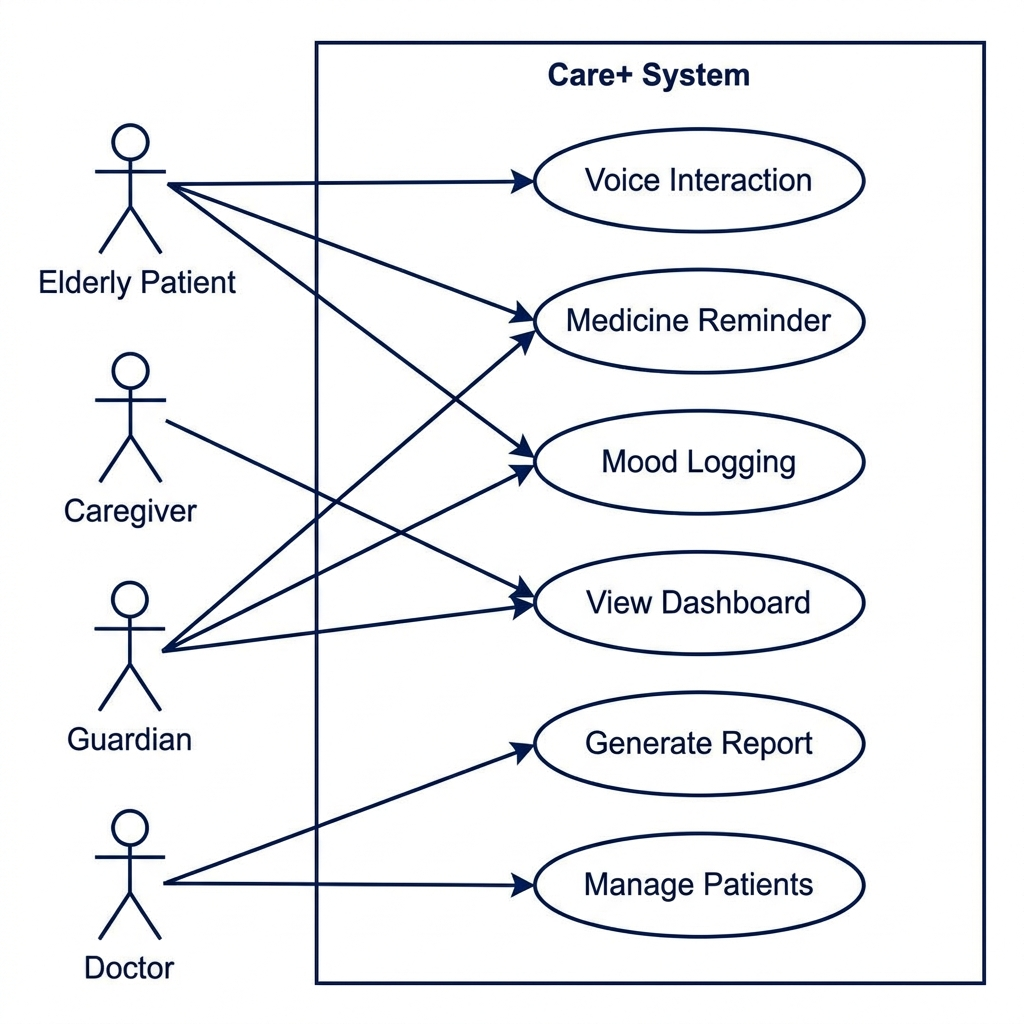
\includegraphics[width=0.9\linewidth, height=10.5cm, keepaspectratio]{usecase.png}
  \end{center}
  \vspace{2mm}
  {\small\textit{Fig.~I: Four actors --- Elderly Patient, Caregiver, Guardian,
  and Doctor --- drive Care+'s voice interaction, medicine reminders, mood
  logging, and clinical dashboards.}}
\end{tcolorbox}

\vspace{3mm}

%% SDG Alignment — real badge images
\begin{tcolorbox}[posterbox, title={SDG ALIGNMENT}]
  Care+ directly supports three UN Sustainable Development Goals:
  \vspace{5pt}
  \begin{columns}[c]
    \begin{column}{0.33\linewidth}
      \centering
      
\includegraphics[width=\linewidth, keepaspectratio]{sdg3.jpg}\\[3pt]
      {\footnotesize\textit{Primary SDG}}
    \end{column}
    \begin{column}{0.33\linewidth}
      \centering
      
\includegraphics[width=\linewidth, keepaspectratio]{sdg9.jpg}\\[3pt]
      {\footnotesize\textit{Innovation}}
    \end{column}
    \begin{column}{0.33\linewidth}
      \centering
      
\includegraphics[width=\linewidth, keepaspectratio]{sdg10.jpg}\\[3pt]
      {\footnotesize\textit{Equity}}
    \end{column}
  \end{columns}
  \vspace{3pt}
  {\small Improves \textbf{medication adherence} \& wellbeing monitoring
  (SDG~3); applies edge-AI innovation for under-served communities (SDG~9);
  bridges Nepal's digital health divide (SDG~10).}
\end{tcolorbox}

\end{column}
\hfill

%% ════════════════════════════════════════
%%  COLUMN 2
%% ════════════════════════════════════════
\begin{column}{0.34\linewidth}
\vspace{3mm}

%% System Architecture
\begin{tcolorbox}[posterbox, title={SYSTEM ARCHITECTURE}]
  \begin{center}
    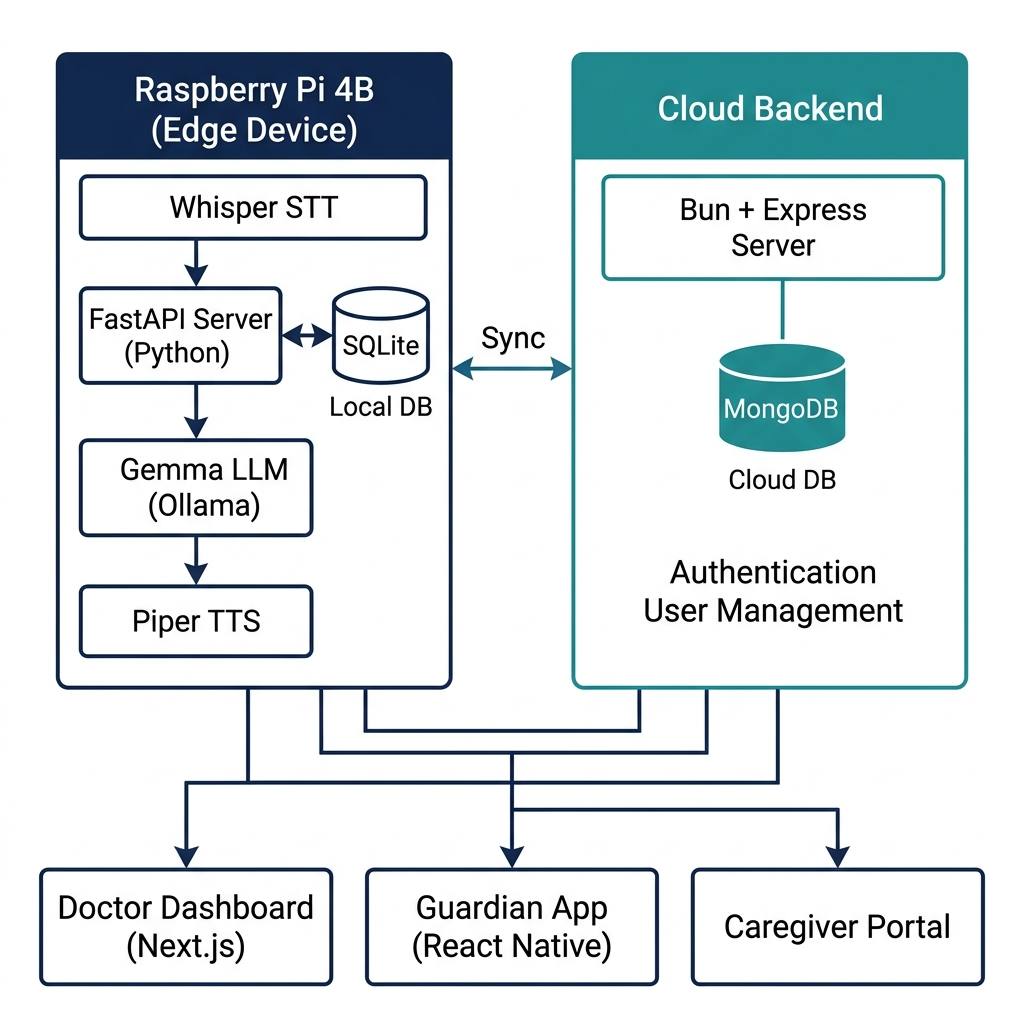
\includegraphics[width=\linewidth, height=15.5cm, keepaspectratio]{arch.png}
  \end{center}
  {\small\textit{Fig.~II: FastAPI + SQLite on Raspberry Pi edge; Bun + Express
  + MongoDB for cloud auth and user management.}}

  \vspace{4mm}

  \renewcommand{\arraystretch}{1.35}
  \begin{tabularx}{\linewidth}{>{\bfseries\color{navyblue}}l X}
    \rowcolor{tableheadbg}
    \color{white}\bfseries Component & \color{white}\bfseries Technology \\
    \rowcolor{rowB} Edge Device      & Raspberry Pi 4B \\
    \rowcolor{rowA} AI / LLM         & Ollama --- Gemma 4 (e2b) \\
    \rowcolor{rowB} Speech-to-Text   & Whisper (Nepali fine-tuned) \\
    \rowcolor{rowA} Text-to-Speech   & Piper TTS (Nepali models) \\
    \rowcolor{rowB} AI API Server    & FastAPI (Python 3.10+) \\
    \rowcolor{rowA} Local Database   & SQLite (on FastAPI server) \\
    \rowcolor{rowB} Cloud Backend    & Bun + Express (TypeScript) \\
    \rowcolor{rowA} Cloud Database   & MongoDB Atlas \\
    \rowcolor{rowB} Mobile App       & React Native (Expo) \\
    \rowcolor{rowA} Web Dashboard    & Next.js \\
  \end{tabularx}
  \renewcommand{\arraystretch}{1}

  \vspace{2mm}
  {\small\textit{Fig.~III: Technology Stack}}
\end{tcolorbox}

\vspace{3mm}

%% Core Interaction Loop
\begin{tcolorbox}[posterbox, title={CORE INTERACTION LOOP}]
  \flowstep{1}{User speaks naturally in \textbf{Nepali or English}}
  \flowstep{2}{\textbf{Whisper STT} converts speech to text on-device}
  \flowstep{3}{\textbf{FastAPI} orchestrates request to local LLM}
  \flowstep{4}{\textbf{Gemma + RAG} determines intent: reply / medicine / mood}
  \flowstep{5}{\textbf{Piper TTS} synthesises a natural Nepali speech response}
  \flowstep{6}{Events persisted to \textbf{SQLite} \& synced to \textbf{MongoDB} via Bun}
  \vspace{2mm}
  {\small\textit{Fig.~IV: Core Interaction Loop}}
\end{tcolorbox}

\vspace{3mm}

%% Mascot / value-proposition illustration
\begin{tcolorbox}[posterbox, title={MEET CARE+}]
  \begin{columns}[c]
    \begin{column}{0.34\linewidth}
      \centering
      
\includegraphics[width=\linewidth, height=8.5cm, keepaspectratio]{robot_cropped.png}
    \end{column}
    \begin{column}{0.66\linewidth}
      {\normalsize A friendly on-device voice companion that speaks Nepali,
      remembers every medicine, and quietly reassures the whole family ---
      \textbf{no cloud, no typing, no language barrier.}}
    \end{column}
  \end{columns}
\end{tcolorbox}

\end{column}
\hfill

%% ════════════════════════════════════════
%%  COLUMN 3
%% ════════════════════════════════════════
\begin{column}{0.315\linewidth}
\vspace{3mm}

%% App Screenshots
\begin{tcolorbox}[posterbox, title={APP SCREENSHOTS --- LIVE MVP}]
  \begin{columns}[t]
    \begin{column}{0.32\linewidth}
      \centering
      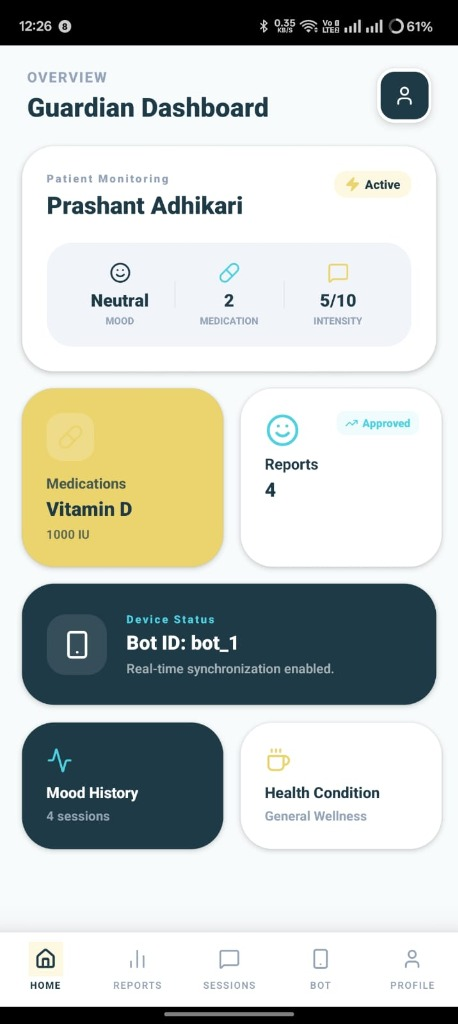
\includegraphics[width=\linewidth, height=12cm, keepaspectratio]{screen_guardian.jpg}
      \vspace{2pt}{\small\bfseries Guardian App}
    \end{column}
    \begin{column}{0.32\linewidth}
      \centering
      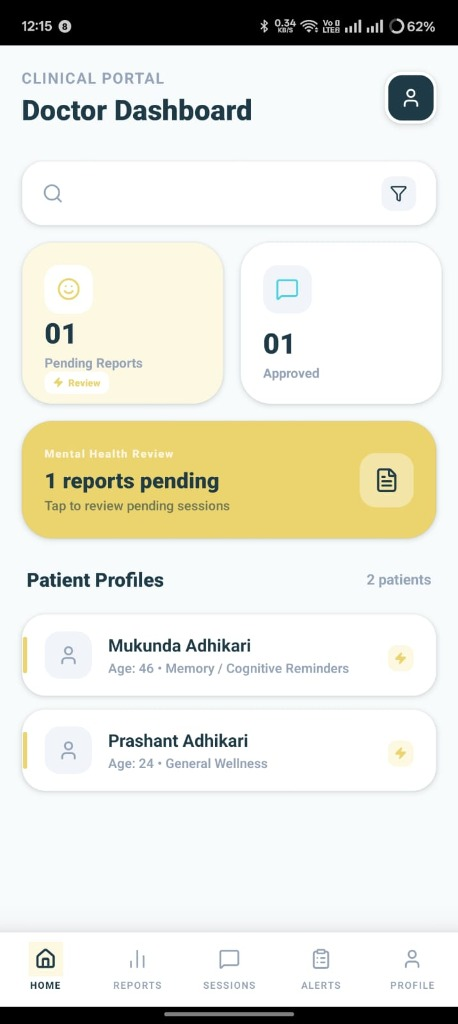
\includegraphics[width=\linewidth, height=12cm, keepaspectratio]{screen_doctor.jpg}
      \vspace{2pt}{\small\bfseries Doctor Portal}
    \end{column}
    \begin{column}{0.32\linewidth}
      \centering
      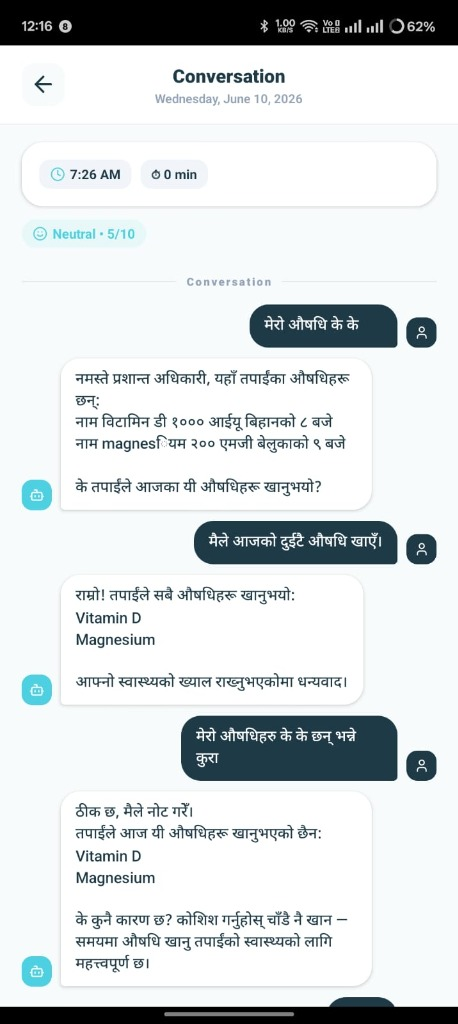
\includegraphics[width=\linewidth, height=12cm, keepaspectratio]{screen_chat.jpg}
      \vspace{2pt}{\small\bfseries AI Chat (Nepali)}
    \end{column}
  \end{columns}
  \vspace{2mm}
  {\small\textit{Fig.~V: Guardian Dashboard, Doctor Clinical Portal, and
  Nepali-language AI Conversation.}}
\end{tcolorbox}

\vspace{3mm}

%% Results
\begin{tcolorbox}[posterbox, title={RESULTS \& TESTING}]
  Validated through unit testing, hardware reliability testing, voice
  recognition across environments, and informal user-acceptance testing
  with elderly pilot participants.
  \vspace{4pt}

  \resultbar{Medicine Reminder Delivery Success}{92}{navyblue}
  \resultbar{Voice Recognition Accuracy (quiet env.)}{88}{midblue}
  \resultbar{Dashboard Sync Reliability}{95}{teal}
  \resultbar{Elderly Preference: Voice over Text App}{85}{sdg9col}

  {\small\textit{Fig.~VI: MVP Performance Indicators (Informal Pilot)}}
\end{tcolorbox}

\vspace{3mm}

%% Methodology
\begin{tcolorbox}[posterbox, title={METHODOLOGY --- AGILE MILESTONES}]
  \begin{columns}[t]
    \begin{column}{0.48\linewidth}
      \msnode{M1}{AI Orchestration}{Whisper + Piper + LLM server routing}
    \end{column}
    \begin{column}{0.48\linewidth}
      \msnode{M2}{Medical Mgmt.}{Medicine CRUD, intake confirmation}
    \end{column}
  \end{columns}
  \vspace{3pt}
  \begin{columns}[t]
    \begin{column}{0.48\linewidth}
      \msnode{M3}{Emotional Analytics}{Mood tracking \& PDF reports}
    \end{column}
    \begin{column}{0.48\linewidth}
      \msnode{M4}{Multi-User Ecosystem}{RPi hardening \& role dashboards}
    \end{column}
  \end{columns}
\end{tcolorbox}

\vspace{3mm}

%% Conclusion
\begin{tcolorbox}[posterbox, title={CONCLUSION \& FUTURE SCOPE}]
  \begin{itemize}
    \item Care+ proves a culturally relevant AI health companion is buildable
      within an academic timeframe.
    \item Local AI eliminates cloud dependency --- critical for Nepal's
      connectivity landscape.
    \item Voice was significantly more accessible to elderly users than
      text-based apps.
    \item \textbf{Future:} Wearable integration, clinical validation,
      expanded South Asian language support, Kathmandu Valley pilot.
  \end{itemize}
\end{tcolorbox}

\vspace{3mm}

%% References
\begin{tcolorbox}[posterbox, title={REFERENCES}]
  {\footnotesize
    [1] ADI. \textit{World Alzheimer Report 2023.}\;
    [2] Radford et al. \textit{Whisper}, ICML 2023.\;
    [3] Nepal CBS. \textit{National Census 2021.}\;
    [4] WHO. \textit{Ageing \& Health}, 2022.\;
    [5] Rhasspy. \textit{Piper TTS}. github.com/rhasspy/piper.}
\end{tcolorbox}

\end{column}
\end{columns}
\end{frame}
\end{document}
